% Financial Innovation (Springer) research article draft.
% Built with the standard article class so it compiles locally; port to the Springer Nature
% LaTeX template (sn-jnl, sn-basic reference style) before submission. See README.md.
\documentclass[11pt]{article}
\usepackage[utf8]{inputenc}
\usepackage[T1]{fontenc}
\usepackage{lmodern}
\usepackage[margin=1in]{geometry}
\usepackage{setspace}
\usepackage{amsmath,amssymb,bm}
\usepackage{booktabs,multirow,makecell}
\usepackage{graphicx}
\usepackage{xcolor}
\usepackage[round,authoryear]{natbib}
\usepackage[hidelinks]{hyperref}
\usepackage{lineno}

\onehalfspacing
\linenumbers

% Draft markers: every \todo must be resolved before submission (grep '\\todo').
\newcommand{\todo}[1]{\textcolor{red}{[TODO: #1]}}
\newcommand{\pending}[1]{\textcolor{blue}{[pending: #1]}}

\newcommand{\Om}{\bm{\Omega}}
\newcommand{\Sig}{\bm{\Sigma}}
\newcommand{\bq}{\bm{q}}
\newcommand{\bmu}{\bm{\mu}}
\newcommand{\bw}{\bm{w}}

\title{Repeated LLM Forecasts as Black--Litterman Views: \\ A Point-in-Time Re-examination of the Dispersion-to-Confidence Mapping}

\author{%
  Youngbin Lee\textsuperscript{1,*} \and Yejin Kim\textsuperscript{2,*} \and Juhyeong Kim\textsuperscript{3} \and Suin Kim\textsuperscript{1} \and
  Yoontae Hwang\textsuperscript{4,\dag} \and Yongjae Lee\textsuperscript{5,\dag}\\[4pt]
  \small \textsuperscript{1}Elice, Seoul, Republic of Korea \quad
  \textsuperscript{2}Meritz Fire \& Marine Insurance, Seoul, Republic of Korea \quad
  \textsuperscript{3}\todo{affiliation} \\
  \small \textsuperscript{4}Pusan National University \quad
  \textsuperscript{5}UNIST \quad
  \textsuperscript{*}Equal contribution \quad \textsuperscript{\dag}Corresponding authors \\
  \small \todo{confirm author list and affiliations for the FI submission}
}
\date{}

\begin{document}
\maketitle

\begin{abstract}
\noindent
Large language models give a different return forecast each time they are asked. An earlier version of this work proposed to turn this into Black--Litterman inputs: the mean of repeated forecasts as the view and their variance as the view uncertainty $\Omega$, so that the forecaster supplies its own confidence. We re-examine this framework with point-in-time index membership from CRSP, open-weight models tested strictly after their documented training cutoffs, and an out-of-sample choice of the scale parameter $\tau$. We also make the framework's claim testable. Because realized returns contain noise that usually exceeds the view error, calibration must be judged against the predictive variance, and because dispersion grows with volatility, the relevant benchmark is the He--Litterman $\Omega$, not a constant. Two tests were fixed in advance: dispersion is informative about view error beyond volatility, and the dispersion-based $\Omega$ improves the portfolio over conventional choices. For the S\&P~500 in 2025 with gpt-oss-20b, the first test passes (volatility-standardized rank correlation 0.12 within dates, positive on 79\% of dates) and the second fails: the dispersion-based $\Omega$ lowers the Sharpe ratio relative to both the constant and the He--Litterman $\Omega$ under level matching, weight caps, recalibration, alternative risk aversion and transaction costs. Dispersion ranks views roughly correctly but spreads their confidence over two orders of magnitude while their errors differ about fourfold, concentrating the portfolio on views that are not more accurate. With returns as the only input, the views themselves are a transformation of short-term momentum without predictive value. The original performance gains do not survive the corrected design. \pending{update with all markets and models}

\medskip\noindent\textbf{Keywords:} Black--Litterman model; large language models; view uncertainty; forecast calibration; portfolio optimization; look-ahead bias
\end{abstract}

\section{Introduction}\label{sec:intro}

The Black--Litterman model \citep{black1992global} is the standard way to bring investor views into a mean--variance portfolio without the instability of plugging forecasts directly into the optimizer \citep{best1991sensitivity,chopra1993effect}. It needs two inputs per view: the view itself and a statement of how much to trust it, the view uncertainty $\Om$. Practice offers little guidance on the second input. It is usually set by convention, proportional to the asset's variance \citep{he2002intuition}, or elicited as a subjective confidence level \citep{idzorek2007step}.

Large language models (LLMs) produce return forecasts on request \citep{lopez2023can,kim2023if}, and they produce a different forecast each time they are asked. An earlier, unpublished version of this work proposed to use both properties\todo{decide how to refer to the EAAI 2026 submission; it is unpublished}: query the model $N$ times for the same stock and date, take the mean of the answers as the view $q_i$ and their variance as the view uncertainty $\Omega_{ii}$. The appeal is that the forecaster supplies its own confidence, so the input that practice leaves to convention becomes measurable, auditable and scalable across assets. That version reported that Black--Litterman portfolios built this way outperformed equal-weight and mean--variance benchmarks on a large-cap US universe.

This paper re-examines that framework. We change three things that could have produced the earlier result. First, data: the universe is rebuilt at every rebalancing date from point-in-time index membership and market capitalizations in CRSP, removing survivorship and look-ahead in stock selection. Second, models: we use only open-weight LLMs with documented training cutoffs and test strictly after them. Third, evaluation: the Black--Litterman scale parameter $\tau$ is chosen out of sample by a walk-forward rule, and every alternative uses the same rule.

We also make the framework's claim testable. The mapping is useful only if the dispersion it uses as $\Om$ tells the investor which views to trust. We show that evaluating this requires two corrections that the earlier study and much of the LLM-uncertainty literature omit. The realized return differs from the expected return by noise whose variance usually exceeds the view error, so calibration must be judged against the predictive variance $s_i^2+\sigma_i^2/h$, not $s_i^2$ alone. LLM dispersion is also larger for volatile stocks, so the right benchmark is not a constant $\Om$ but the He--Litterman $\Om$, which already scales with volatility. Before running the out-of-sample collection we fixed two tests: (a) dispersion is associated with view error beyond volatility, and (b) holding the views fixed, the dispersion-based $\Om$ gives a better portfolio than the constant and He--Litterman $\Om$.

In the US pilot (S\&P~500, gpt-oss-20b, 2025) test (a) passes and test (b) fails. Dispersion does carry information about forecast error beyond volatility: the within-date rank correlation after volatility standardization is 0.12, positive on 79\% of dates. Used as $\Om$, however, it lowers the Sharpe ratio relative to both conventions in every specification we try, including level matching, a 10\% weight cap, recalibration, four values of the risk-aversion parameter and four cost levels. The reason is a mismatch of magnitudes. Dispersion ranks views roughly correctly but spreads them over two orders of magnitude, while their actual errors differ by a factor of about four, mostly because of volatility. The mapping therefore concentrates the portfolio on a few views that are not more accurate. Behind this lies a more basic finding: with returns as the only input, the model's views are a transformation of short-term momentum (rank correlation 0.96) and have no predictive value at the two-week horizon. With uninformative views no choice of $\Om$ can add value, and one that concentrates does harm.

The paper makes three contributions. First, it provides a point-in-time, cutoff-clean re-examination of the LLM-to-Black--Litterman framework, and shows that the original performance result does not survive it. Second, it gives an evaluation protocol for any source of Black--Litterman view uncertainty: decompose forecast error into view error and return noise, separate shape from level using the $\tau$--$\Om$ invariance, benchmark against He--Litterman, and choose $\tau$ out of sample. Third, it documents why a dispersion signal that is informative in rank can still be harmful as $\Om$, which bears on the broader use of sampled LLM disagreement as a confidence measure in financial decisions.

Section~\ref{sec:related} reviews related work. Section~\ref{sec:framework} states the framework and the tests, Section~\ref{sec:data} the data and design, Section~\ref{sec:results} the results, and Section~\ref{sec:discussion} their implications and limits.

\section{Related literature}\label{sec:related}

\paragraph{Views and confidence in Black--Litterman.}
Mean--variance weights are highly sensitive to errors in expected returns \citep{best1991sensitivity,chopra1993effect,michaud1989markowitz}, and estimation risk motivates Bayesian and shrinkage approaches \citep{jorion1986bayes,pastor2000portfolio,garlappi2007portfolio,demiguel2009optimal}. \citet{black1992global} anchor expected returns at the equilibrium implied by market weights and tilt them toward investor views in proportion to view confidence. Confidence is the least specified input. \citet{he2002intuition} set $\Om$ proportional to the prior variance of the view portfolio, $\tau\bm{P}\Sig\bm{P}^\top$, so that confidence is tied to volatility and the ratio of view to prior weight is the same for every view. \citet{idzorek2007step} instead asks the investor for a percentage confidence in each view and backs out $\Omega_{ii}$ from it. \citet{satchell2007demystification} and \citet{walters2014black} review the role of $\tau$ and $\Om$ and note that only their ratio is identified. In all of these, the confidence is either a convention or an opinion. The mapping studied here proposes a third source: the dispersion of a model's own repeated forecasts.

\paragraph{LLMs as return forecasters.}
\citet{lopez2023can} show that ChatGPT's reading of news headlines predicts next-day returns, and \citet{kim2023if} use an LLM to choose asset allocations from macroeconomic narratives; \citet{romanko2023chatgpt} use it to select stocks. Most such work uses the model's output as a signal for sorting or as a direct allocation, and does not produce the confidence input that a Bayesian allocator needs. A second line of work warns that LLM forecasts on historical data can be contaminated by training on later text \citep{glasserman2023assessing,sarkar2024lookahead}; \citet{drinkall2024time} train models with strict temporal cutoffs for this reason. We restrict the test period to dates after documented cutoffs.

\paragraph{Uncertainty from LLM outputs.}
In natural language processing, the spread of repeated samples is a common uncertainty signal: agreement among sampled answers improves reasoning accuracy \citep{wang2023selfconsistency}, inconsistency among samples flags hallucination \citep{manakul2023selfcheckgpt}, and semantic dispersion predicts error \citep{kuhn2023semantic}. Verbalized and sampled confidence can be informative but is often overconfident \citep{kadavath2022language,lin2022teaching,xiong2024can}. These studies evaluate classification or question answering, where correctness is observed directly. In return forecasting the target, the expected return, is never observed, and realized returns are dominated by noise. Section~\ref{sec:requirements} shows that this changes how sampled dispersion must be evaluated.

\paragraph{Short-horizon return patterns.}
At horizons of one week to one month, individual stock returns show reversal rather than continuation \citep{jegadeesh1990evidence,lehmann1990fads}. A forecaster that extrapolates the last two weeks is therefore expected to lose at the two-week horizon used here, which matters for interpreting Section~\ref{sec:res_q}.

\paragraph{Evaluation practice.}
Survivorship and look-ahead in the asset universe inflate backtested performance \citep{brown1992survivorship,elton1996survivorship}. Sharpe ratio differences between overlapping strategies require tests that respect serial dependence \citep{ledoit2008robust}. Probabilistic forecasts are judged by calibration and proper scoring rules \citep{gneiting2007strictly}.

\section{Framework}\label{sec:framework}

This section restates the Black--Litterman update, defines the mapping from repeated LLM forecasts to its inputs, and states what that mapping must satisfy to be useful. The last part turns those requirements into two tests that we fixed before running the out-of-sample experiments.

\subsection{Black--Litterman with absolute views}
At a rebalancing date the investor holds $n$ assets with covariance matrix $\Sig$ and market-capitalization weights $\bw_m$. The equilibrium prior for expected excess returns is
\begin{equation}
  \bmu \sim \mathcal{N}(\bm{\Pi}, \tau\Sig), \qquad \bm{\Pi} = \delta \Sig \bw_m ,
\end{equation}
where $\delta$ is the market's risk aversion and $\tau$ scales the uncertainty of the prior \citep{black1992global,he2002intuition}. The investor states one absolute view per asset ($\bm{P}=\bm{I}$),
\begin{equation}
  \bq = \bmu + \bm{\varepsilon}, \qquad \bm{\varepsilon} \sim \mathcal{N}(\bm{0}, \Om), \quad \Om = \mathrm{diag}(\Omega_{11},\dots,\Omega_{nn}),
\end{equation}
and the posterior mean is
\begin{equation}\label{eq:posterior}
  \bmu_{BL} = \left[(\tau\Sig)^{-1} + \Om^{-1}\right]^{-1}\left[(\tau\Sig)^{-1}\bm{\Pi} + \Om^{-1}\bq\right].
\end{equation}
Weights solve the long-only problem $\min_{\bw}\ \bw^\top\Sig\bw - \lambda\,\bw^\top\bmu_{BL}$ subject to $\bm{1}^\top\bw = 1$ and $0 \le w_i \le w_{\max}$, with $\lambda = 0.1$ as in the original study and $w_{\max}=1$ unless stated otherwise.

$\Omega_{ii}$ is the variance of the view error $q_i - \mu_i$: how far the stated view can be from the true expected return. Equation~\eqref{eq:posterior} uses $\Omega_{ii}^{-1}$ as the weight on view $i$. A source of $\Om$ is therefore useful only if views that it labels as uncertain are, on average, further from $\mu_i$.

\subsection{From repeated forecasts to $(\bq, \Om)$}
For asset $i$ at a rebalancing date we send the same prompt $N$ times and record numerical forecasts $y_{i1},\dots,y_{iN}$ of the asset's average daily return over the next two weeks. The mapping of the original study is
\begin{equation}\label{eq:mapping}
  q_i = \bar y_i = \frac{1}{N}\sum_{k=1}^N y_{ik}, \qquad \Omega_{ii} = s_i^2 = \frac{1}{N-1}\sum_{k=1}^N (y_{ik}-\bar y_i)^2 .
\end{equation}
$s_i^2$ is not divided by $N$, because it is read as the model's uncertainty about the view, not as the sampling error of $\bar y_i$. We call this the \emph{empirical} $\Om$.

\subsection{What the mapping must satisfy}\label{sec:requirements}
$\mu_i$ is never observed. What we observe is the realized average daily return over the holding period, $\bar r_i = \mu_i + \eta_i$, where $\eta_i$ is return noise with variance close to $\sigma_i^2/h$ for daily volatility $\sigma_i$ and $h$ trading days. If the view error and the noise are independent,
\begin{equation}\label{eq:decomp}
  \mathbb{E}\left[(q_i - \bar r_i)^2\right] = \underbrace{\mathbb{E}\left[(q_i-\mu_i)^2\right]}_{\text{view error, the target of } \Omega_{ii}} + \underbrace{\sigma_i^2/h}_{\text{return noise}} .
\end{equation}
Equation~\eqref{eq:decomp} has two consequences for evaluation.

\paragraph{Level.} A nominal 95\% interval built from $s_i^2$ alone will cover $\bar r_i$ far less than 95\% of the time even when $s_i^2$ is exactly right, because it ignores $\sigma_i^2/h$. The correct check uses the predictive variance $s_i^2 + \sigma_i^2/h$. More importantly for the portfolio, the overall level of $\Om$ is not identified separately from $\tau$: from \eqref{eq:posterior}, $\bmu_{BL}(c\tau, c\Om) = \bmu_{BL}(\tau,\Om)$ for any $c>0$. A $\tau$ chosen out of sample (Section~\ref{sec:tau}) absorbs any uniform over- or under-confidence. What $\tau$ cannot absorb is variation of the level from one rebalancing date to the next, because $\tau$ is held fixed within a quarter.

\paragraph{Shape.} What the mapping must deliver is the cross-sectional \emph{shape} of $\Om$: whether assets with larger $s_i^2$ have larger view error. The expected squared error in \eqref{eq:decomp} grows with $\sigma_i^2$ through the noise term, and LLM forecasts for volatile stocks are also more dispersed. A raw rank correlation between $s_i^2$ and squared error can therefore be produced by volatility alone. The relevant comparator is the He--Litterman convention $\Omega_{ii} \propto \tau\Sig_{ii}$ \citep{he2002intuition}, which already encodes volatility. After rescaling both to the same average level, the empirical $\Om$ differs from He--Litterman exactly by the volatility-standardized dispersion $s_i^2/\Sig_{ii}$. The question ``does LLM dispersion carry information about view error beyond volatility?'' is the same as ``does the empirical $\Om$ beat He--Litterman?''

\subsection{Variants of $\Om$}\label{sec:omega_variants}
All variants use the same $\bq$, so differences in portfolio outcomes come from $\Om$ only.
\begin{itemize}
  \item \textbf{Empirical}: $\Omega_{ii} = s_i^2$ (Eq.~\ref{eq:mapping}).
  \item \textbf{Constant}: $\Omega_{ii} = \frac{1}{n}\sum_j s_j^2$. Same level as empirical, no cross-sectional shape.
  \item \textbf{Shuffled}: the values $s_j^2$ randomly permuted across assets. Same distribution, wrong assignment.
  \item \textbf{He--Litterman}: $\Omega_{ii} = \tau \Sig_{ii}$.
  \item \textbf{Isotonic-calibrated}: $\Omega_{ii} = g(s_i^2)$ with $g$ a monotone map from $\log s^2$ to realized squared error, fitted by isotonic regression on earlier forecast--outcome pairs only.
  \item \textbf{Linear-calibrated}: $\Omega_{ii} = \max(a + b\,s_i^2, \epsilon)$, with $(a,b)$ from least squares of the noise-adjusted squared error $(q_j-\bar r_j)^2 - \hat\sigma_j^2/h$ on $s_j^2$ over earlier pairs, $b\ge 0$. This targets the view error in \eqref{eq:decomp} directly.
\end{itemize}
We report each variant under four specifications: as defined (\emph{raw}); \emph{level-matched}, where $\Om$ is rescaled at each date so that its cross-sectional mean equals $\tau\cdot\frac{1}{n}\sum_i\Sig_{ii}$, which removes the date-to-date level variation that $\tau$ cannot absorb and leaves only shape; with a 10\% per-asset weight cap; and with both.

\subsection{Choosing $\tau$ out of sample}\label{sec:tau}
For each strategy that has a $\tau$, we compute weight paths for 13 values of $\tau$ on a log grid from $10^{-3}$ to $10$. At the start of each calendar quarter we pick the $\tau$ with the highest Sharpe ratio over all earlier holding periods (expanding window, net of costs) and use it for that quarter. The first two quarters are used only to make the first choice and are not evaluated. Calibration maps are fitted with the same expanding window. Every comparison below therefore uses the same, fully out-of-sample procedure; no parameter is tuned on the evaluation period as a whole.

\subsection{Pre-specified tests}\label{sec:criteria}
Before running the out-of-sample LLM collection we fixed two tests of the framework in the project's design document. Comparisons with naive or momentum portfolios are reported but are not part of the tests, because the framework's claim concerns the mapping, not the return forecasting skill of a particular model.
\begin{enumerate}
  \item[(a)] \textbf{Information}: $s_i^2$ is associated with view error beyond volatility. Measured by the Spearman correlation between $s_i^2/\hat\sigma_i^2$ and $(q_i-\bar r_i)^2/\hat\sigma_i^2$, its within-date average, and the partial rank correlation given $\hat\sigma_i^2$.
  \item[(b)] \textbf{Decision value}: with the same $\bq$, the empirical $\Om$ yields a higher out-of-sample Sharpe ratio than the constant and the He--Litterman $\Om$.
\end{enumerate}

\section{Data and experimental design}\label{sec:data}

\subsection{Point-in-time data}
Returns, market capitalizations and index membership come from WRDS: CRSP daily stock files for the S\&P~500 (total returns including dividends) and Compustat Global for the KOSPI~200, Nikkei~225 and DAX, from January 2000 to 31 December 2025. Each security carries the dates on which it entered and left the index, so the constituent list on any date can be rebuilt. The risk-free rate is the three-month Treasury bill (FRED \texttt{DTB3}) for the United States and the OECD three-month interbank rate for the other markets.

The original study used a fixed list of stocks chosen from today's index with today's market capitalizations. That design has two biases. Survivorship: firms that left the index during the test period are missing \citep{brown1992survivorship,elton1996survivorship}. Look-ahead in the universe: the selection uses information from after the decision date. Here the universe at each rebalancing date is the 50 largest index members \emph{on that date} by market capitalization \emph{on that date}. Stocks that leave the index drop out at the next rebalancing; new entrants are added and receive LLM forecasts from then on. Over the US test period 64 distinct stocks enter the universe.

\subsection{Period and models}
The test period has to start after the training cutoff of every model used and end before the data end. We use only open-weight models whose developers document the training cutoff \todo{cite docs/R4 table in appendix}: gpt-oss-20b and gpt-oss-120b (June 2024) \citep{openai2025gptoss}, Gemma~3 27B (August 2024) \citep{team2025gemma3} and Llama~3.3 70B (December 2023) \citep{meta2024llama33}. Models with undocumented or later cutoffs are excluded, because a forecast for a period the model has read about is not a forecast \citep{glasserman2023assessing,sarkar2024lookahead}. This leaves 1 September 2024 to 31 December 2025: 35 two-week rebalancing periods per market. The first two quarters (September--December 2024) serve only for the first choice of $\tau$; evaluation covers the 26 rebalancing decisions from January to December 2025 (239 trading days), which include the April 2025 tariff sell-off.

This version of the paper reports the pilot market and model: the S\&P~500 with gpt-oss-20b. \pending{KOSPI 200, Nikkei 225, DAX; gpt-oss-120b, Gemma 3 27B, Llama 3.3 70B; prompt B.}

\subsection{Forecast collection}
For each stock and rebalancing date the model receives the stock's name and ticker, its daily returns over the last ten trading days, and the cap-weighted daily returns of the universe over the same days (prompt A, which keeps the information set of the original study). It is asked for the average daily return in percent over the next ten trading days and returns a single number (Appendix~\ref{app:prompt}). Each prompt is sent $N=20$ times at temperature 1.0. gpt-oss-20b is a reasoning model; we use low reasoning effort. Models are served locally with vLLM \citep{kwon2023efficient} on one NVIDIA H100 GPU. The US collection produced 34{,}762 forecasts for 1{,}750 stock-dates; 0.7\% of responses could not be parsed and are dropped (19.9 valid draws per stock-date on average). Collection took 4.5 GPU-hours.

\subsection{Portfolio construction and evaluation}
$\Sig$ is the Ledoit--Wolf shrinkage estimate \citep{ledoit2004well} from the last 126 trading days. $\delta = 2.5$ \citep{he2002intuition}; Section~\ref{sec:robust} reports $\delta \in \{1.5, 3.5\}$ and a trailing 252-day estimate. Weights are set at the end of each period, drift with prices during the next two weeks, and the one-way turnover against the drifted weights is charged 10 basis points on the first holding day (0, 5 and 25 bp in the appendix).

Comparisons that share $\bq$ and differ only in $\Om$ answer test (b). We also report, as reference points, portfolios that do not use LLM views: equal weight, market-cap weight, long-only mean--variance on the 126-day mean, the Black--Litterman prior alone (no views), Black--Litterman with a momentum view ($\bq$ = trailing ten-day mean return, constant $\Om$), Black--Litterman with the 126-day mean as view and its sampling variance as $\Om$, and an equal-weighted top-ten momentum portfolio. Two LLM portfolios without Black--Litterman isolate the role of the update: mean--variance on $\bq$ directly, and equal weight on the ten stocks with the highest $q_i$.

Differences in annualized Sharpe ratio are tested with a paired circular block bootstrap \citep{politis1992circular,ledoit2008robust} on daily excess returns (block length 10 days, 2{,}000 resamples), which resamples the same dates for both portfolios. We report the difference, its 95\% percentile interval and a two-sided bootstrap $p$-value.

For test (a) each stock-date yields one forecast--outcome pair $(q_i, s_i^2, \bar r_i, \hat\sigma_i^2)$, where $\hat\sigma_i^2$ is the 126-day variance of daily returns known at the decision date. The US pilot has 1{,}700 pairs over 34 dates.

\section{Results}\label{sec:results}

All numbers in this section are for the S\&P~500 with gpt-oss-20b, prompt A, $N=20$, evaluated over the 26 rebalancing decisions of 2025. \pending{Other markets and models will be added as columns or panels of the same tables.}

\subsection{What the views contain}\label{sec:res_q}
Table~\ref{tab:q} describes $\bq$ before it enters the portfolio. The cross-sectional ranking of $q_i$ is almost the ranking of the trailing ten-day return (rank correlation 0.96). Its rank correlation with the next two-week return is 0.02, and the slope of the next return on $q_i$ is slightly negative. Given only recent returns, the model extrapolates them. At the two-week horizon in 2025 that signal had no predictive value; the trailing ten-day mean itself had a rank correlation of 0.01 with the next period. The views are also uniformly optimistic: the average $q_i$ is 0.20\% per day (about 65\% annualized), against a realized average of 0.08\%.

\begin{table}[t]
\centering
\caption{What the LLM views contain. Rank correlations are cross-sectional Spearman correlations computed at each rebalancing date and averaged over the 34 dates. US, gpt-oss-20b, prompt A, $N=20$.}
\label{tab:q}
\small
\begin{tabular}{lr}
\toprule
Quantity & Value \\
\midrule
Rank correlation of $q_i$ with the trailing 10-day mean return & 0.959 \\
Rank correlation of $q_i$ with the next two-week mean return & 0.017 \\
Rank correlation of the trailing 10-day mean with the next two-week mean & 0.012 \\
Slope of the next two-week return on $q_i$ (both demeaned by date) & -0.048 \\
Mean $q_i$ (\% per day) & 0.200 \\
Mean realized return (\% per day) & 0.080 \\
\bottomrule
\end{tabular}

\end{table}

\subsection{Test (a): is dispersion informative about view error?}\label{sec:res_a}
Table~\ref{tab:calib} reports the shape and level diagnostics of Section~\ref{sec:criteria}. The raw rank correlation between $s_i^2$ and the squared error is 0.19. Part of it is volatility: dispersion and the trailing variance have a rank correlation of 0.33. After standardizing both by $\hat\sigma_i^2$, the correlation is 0.15; the partial rank correlation given $\hat\sigma_i^2$ is 0.12; computed within each date it averages 0.12, is positive on 79\% of dates and has a $t$-statistic of 4.4 across dates. Test (a) is passed: LLM dispersion carries information about forecast error that volatility does not.

The level diagnostics follow Eq.~\eqref{eq:decomp}. An interval built from $s_i^2$ alone covers the realized return 36\% of the time at the nominal 95\% level. Adding the return-noise variance gives 92.8\%, close to nominal, and the noise variance by itself already gives 91.3\%. On average $s_i^2$ is about one ninth of $\hat\sigma_i^2/h$. Most of the forecast error is return noise that no forecaster could remove, and the ``overconfidence'' of the raw interval is mostly the omitted noise term.

All diagnostics are nearly identical for $N=5$, 10 and 20. The information in dispersion saturates by $N=5$--10, so the number of queries per stock can be cut by half or more without loss.

\begin{table}[t]
\centering
\caption{Dispersion as an uncertainty signal. $e^2=(q_i-\bar r_i)^2$, $\hat\sigma^2$ the trailing 126-day variance, $h$ the number of trading days in the holding period. $N=5$ and $10$ are averages over three random subsets of the 20 draws. Coverage is the share of pairs with $|q_i-\bar r_i| \le 1.96\times$ the stated standard deviation. 1{,}700 pairs over 34 dates.}
\label{tab:calib}
\small
\begin{tabular}{lrrr}
\toprule
 & $N=5$ & $N=10$ & $N=20$ \\
\midrule
$\rho(s^2, e^2)$ & 0.172 & 0.173 & 0.187 \\
$\rho(s^2/\hat\sigma^2, e^2/\hat\sigma^2)$ & 0.148 & 0.141 & 0.150 \\
Partial $\rho$ given $\hat\sigma^2$ & 0.123 & 0.116 & 0.124 \\
Within-date mean & 0.117 & 0.110 & 0.123 \\
Share of dates $>0$ & 0.745 & 0.775 & 0.794 \\
$t$ (across dates) & 4.102 & 4.220 & 4.417 \\
\midrule
95\% cov., $s^2$ & 0.314 & 0.344 & 0.362 \\
95\% cov., $s^2+\hat\sigma^2/h$ & 0.923 & 0.927 & 0.928 \\
95\% cov., $\hat\sigma^2/h$ & 0.909 & 0.912 & 0.913 \\
\bottomrule
\end{tabular}

\end{table}

\subsection{Test (b): does the dispersion improve the portfolio?}\label{sec:res_b}
Table~\ref{tab:omega} and Figure~\ref{fig:omega} hold $\bq$ fixed and vary only $\Om$. Test (b) fails in every specification. The empirical $\Om$ has the lowest Sharpe ratio of all variants in three of the four specifications. It is below the constant $\Om$ by 0.49 to 0.97, significant at 5\% in all four. It is below He--Litterman by 0.51 to 1.15, significant in three of four. Level matching and the 10\% cap raise the Sharpe ratio of every variant except the shuffled one, whose raw value (0.48, from a single random permutation) is the outlier of the table; He--Litterman is unaffected by level matching by construction. Neither changes the conclusion of test (b).

Recalibration removes part of the damage: the linear-calibrated $\Om$ is better than the empirical $\Om$ in all four specifications and the isotonic one in three. Neither beats the conventions. The linear-calibrated $\Om$ is below the constant $\Om$ in all four specifications ($p<0.05$) and significantly below He--Litterman in three. Assigning the same dispersion values to randomly chosen stocks (shuffled) gives a higher Sharpe ratio than assigning them to the right stocks in all four specifications; the difference is significant in the raw specification ($p<0.01$) and marginal under level matching ($p=0.06$).

\begin{table}[t]
\centering
\caption{Annualized Sharpe ratio of Black--Litterman portfolios that share the LLM views $\bq$ and differ only in $\Om$, under four specifications (Section~\ref{sec:omega_variants}). He--Litterman is already at the He--Litterman level, so its level-matched entries equal the unmatched ones. Lower panel: Sharpe ratio differences, paired circular block bootstrap; $^{*}$, $^{**}$, $^{***}$: two-sided $p<0.10, 0.05, 0.01$. 2025, 10 bp costs, $\tau$ chosen out of sample.}
\label{tab:omega}
\small
\begin{tabular}{lrrrr}
\toprule
$\bm{\Omega}$ & Raw & Level-matched & 10\% cap & Level-matched + cap \\
\midrule
Empirical ($s_i^2$) & -2.02 & -1.46 & -0.28 & -0.34 \\
Constant & -1.32 & -0.49 & 0.31 & 0.15 \\
Shuffled & 0.48 & -0.50 & -0.12 & -0.07 \\
He--Litterman ($\tau\Sigma_{ii}$) & -0.87 & -0.87 & 0.23 & 0.23 \\
Isotonic-calibrated & -1.45 & -0.92 & -0.30 & -0.09 \\
Linear-calibrated & -1.81 & -1.00 & -0.25 & -0.07 \\
\midrule
Empirical $-$ Constant & -0.70$^{**}$ & -0.97$^{**}$ & -0.59$^{**}$ & -0.49$^{**}$ \\
Linear-calibrated $-$ Constant & -0.49$^{**}$ & -0.52$^{**}$ & -0.56$^{***}$ & -0.22$^{**}$ \\
Empirical $-$ He--Litterman & -1.15$^{***}$ & -0.58 & -0.51$^{**}$ & -0.57$^{***}$ \\
Linear-calibrated $-$ He--Litterman & -0.94$^{***}$ & -0.13 & -0.48$^{***}$ & -0.30$^{**}$ \\
\bottomrule
\end{tabular}

\end{table}

\begin{figure}[t]
\centering
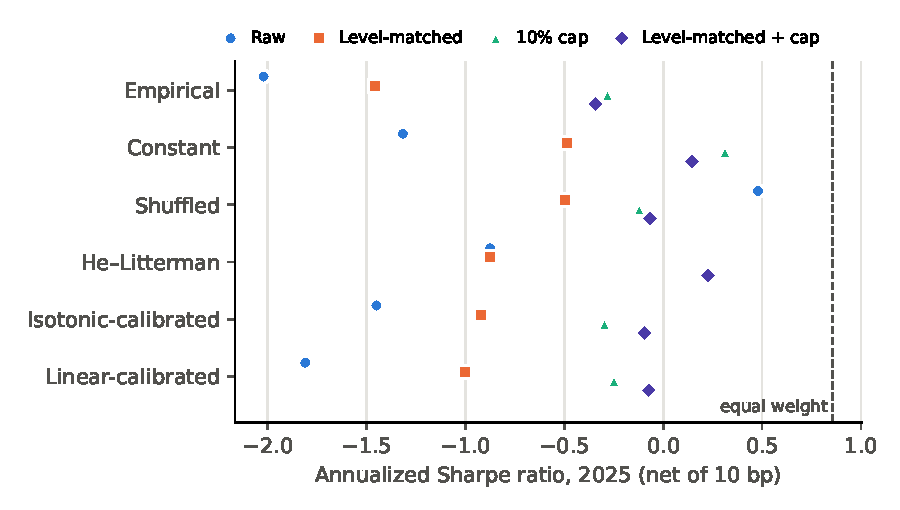
\includegraphics[width=0.85\linewidth]{figures/fig_omega}
\caption{Sharpe ratio of each $\Om$ variant under the four specifications; same data as Table~\ref{tab:omega}. The dashed line is the equal-weight portfolio.}
\label{fig:omega}
\end{figure}

\subsection{Why informative dispersion has negative decision value}\label{sec:res_why}
Tests (a) and (b) disagree. Figure~\ref{fig:deciles} shows why. It sorts stocks into deciles of $s_i^2$ within each date and plots the average dispersion, squared error and return noise per decile. From the lowest to the highest decile, $s_i^2$ rises by a factor of 121. The realized squared error rises by a factor of 4.0, and the return noise, which is pure volatility, by 3.2. Within a single date the 90th percentile of $s_i^2$ is 22 times the 10th percentile; for the trailing variance the ratio is 5.6.

\begin{figure}[t]
\centering
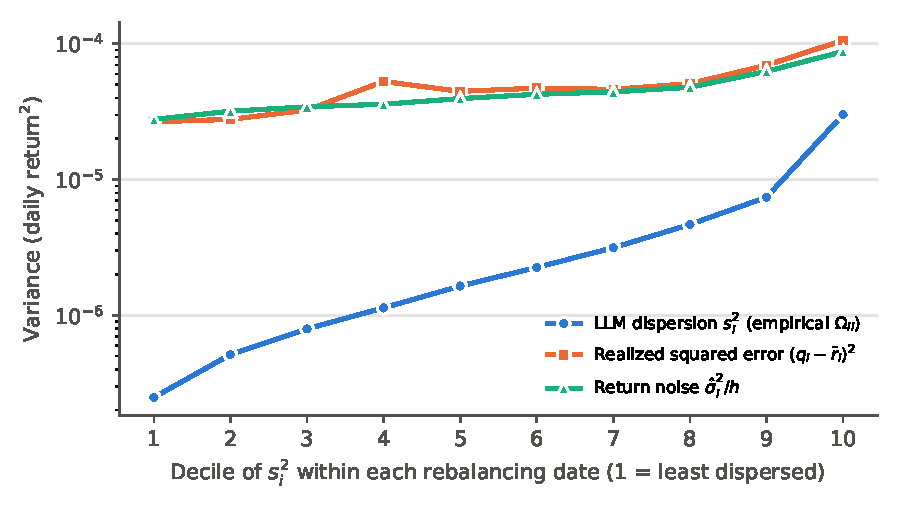
\includegraphics[width=0.85\linewidth]{figures/fig_deciles}
\caption{Dispersion overstates differences in forecast error. Stocks are sorted into deciles of $s_i^2$ within each rebalancing date; lines show decile averages (log scale). The realized squared error tracks the return noise; the dispersion spans two orders of magnitude more.}
\label{fig:deciles}
\end{figure}

The ordering in $s_i^2$ is right on average, but its magnitude is not. Used as $\Om$, the empirical mapping trusts the least dispersed views about a hundred times more than the most dispersed ones, while their actual errors differ by a factor of about four, most of which volatility, and hence He--Litterman, already captures. Because $\bq$ carries no predictive information (Section~\ref{sec:res_q}), concentrating weight on a subset of views only adds variance: the uncapped empirical portfolio puts up to 91\% in one stock. A constant $\Om$ spreads the same views evenly and loses less.

Two features of the draws help explain the exaggerated spread. First, dispersion follows the size of the recent move: the rank correlation between $s_i^2/\hat\sigma_i^2$ and $|$trailing ten-day return$|/\hat\sigma_i$ is 0.52. The model disagrees with itself more when it has a large move to extrapolate, which is also when the extrapolated view is far from a realized return near zero. Second, answers are discrete: the 20 draws for a stock-date contain on average 10 distinct values, the most common value accounts for 29\% of them, and 0.05\% per day alone accounts for 10\% of all 34{,}762 answers. Low dispersion often means the model repeated a round number, not that it was more certain.

We also tested whether the common optimism of $\bq$ drives the result, by shifting all views so that their cross-sectional mean equals that of the prior $\bm{\Pi}$. This leaves the empirical portfolio unchanged ($-2.01$ against $-2.02$; Table~\ref{tab:center} in the appendix). The harm comes from the cross-sectional shape of $\Om$, not from the level of $\bq$.

\subsection{Reference portfolios}\label{sec:res_ref}
Table~\ref{tab:reference} places these results among portfolios without LLM views. Equal weight has a Sharpe ratio of 0.86 and no Black--Litterman portfolio with LLM views comes close; the best is the constant $\Om$ with a 10\% cap (0.31). Black--Litterman with a momentum view behaves like the LLM version ($-1.65$ uncapped), as expected from Table~\ref{tab:q}. The top-ten portfolio by LLM $q_i$ (0.73) and the top-ten momentum portfolio (0.71) are statistically indistinguishable (difference 0.02, $p=0.92$). The original study's finding that LLM views in Black--Litterman beat equal weight does not hold with point-in-time data, a documented-cutoff model and an out-of-sample $\tau$.

\begin{table}[t]
\centering
\caption{Reference portfolios, 2025, 10 bp costs. Max $w$: largest single weight at any rebalancing date. Right block: same strategy with a 10\% weight cap, where it applies.}
\label{tab:reference}
\small
\begin{tabular}{lrrrrr|rr}
\toprule
 & Sharpe & CAGR & Vol. & MDD & Max $w$ & \multicolumn{2}{c}{10\% cap} \\
 & & & & & & Sharpe & MDD \\
\midrule
Equal weight & 0.86 & 0.19 & 0.17 & -0.18 & 0.02 & -- & -- \\
Market-cap weight & 0.79 & 0.21 & 0.21 & -0.21 & 0.13 & -- & -- \\
MVO, 126-day mean & 0.54 & 0.15 & 0.23 & -0.19 & 0.44 & 0.38 & -0.19 \\
BL prior only (no views) & -0.12 & 0.01 & 0.14 & -0.13 & 0.27 & 0.03 & -0.13 \\
BL, 126-day mean view & 0.51 & 0.14 & 0.23 & -0.19 & 0.44 & 0.33 & -0.18 \\
BL, momentum view & -1.65 & -0.36 & 0.27 & -0.44 & 0.86 & 0.05 & -0.14 \\
Top-10 momentum & 0.71 & 0.18 & 0.21 & -0.19 & 0.10 & -- & -- \\
MVO on LLM $q$ & -0.82 & -0.18 & 0.25 & -0.34 & 0.91 & 0.35 & -0.17 \\
Top-10 by LLM $q$ & 0.73 & 0.18 & 0.20 & -0.19 & 0.10 & -- & -- \\
BL, LLM $q$, empirical $\Omega$ & -2.02 & -0.36 & 0.23 & -0.38 & 0.91 & -0.28 & -0.14 \\
BL, LLM $q$, He--Litterman $\Omega$ & -0.87 & -0.17 & 0.23 & -0.30 & 0.65 & 0.23 & -0.15 \\
\bottomrule
\end{tabular}

\end{table}

\subsection{Robustness}\label{sec:robust}
\paragraph{Risk aversion $\delta$.} Table~\ref{tab:delta} in the appendix varies $\delta$ over 1.5, 2.5 and 3.5 and a trailing 252-day estimate $\hat\delta = \mathbb{E}[r_m - r_f]/\mathrm{Var}(r_m)$. The estimate ranges from 3.3 to 18.0 (median 5.6) and is never negative in this window. Sharpe ratios of the Black--Litterman portfolios with views change by at most 0.04, and the ordering of $\Om$ variants and all test conclusions are the same for every $\delta$. $\delta$ only scales $\bm{\Pi}$, and the out-of-sample $\tau$ re-balances prior against views. The prior-only portfolio, which has no views to rebalance against, moves more ($-0.26$ to $-0.04$).

\paragraph{Transaction costs.} From 0 to 25 basis points the ordering of the $\Om$ variants does not change (Table~\ref{tab:costs}).

\paragraph{Choice of $\tau$.} The out-of-sample $\tau$ is unstable: for the raw empirical $\Om$ it moves from 10 in the first quarter to $10^{-3}$ in the last, because early choices rest on four months of data. The 10\% cap is our main safeguard against the resulting concentration. \todo{fixed-split robustness (choose $\tau$ once on Sep--Dec 2024).}

\paragraph{Fixed universe.} \todo{Rerun with the universe fixed at 30 August 2024 to quantify the effect of the point-in-time universe alone.}

\section{Discussion}\label{sec:discussion}

\paragraph{Information is not decision value.}
Test (a) asks whether dispersion ranks view errors correctly; test (b) asks whether it improves the portfolio. The US pilot shows that the first does not imply the second. Black--Litterman uses $\Omega_{ii}^{-1}$ as a weight, so the magnitudes of $\Om$ matter, not only its ordering. A signal with a modest rank correlation but a hundredfold range acts like a strong signal in the optimizer. Recalibration addresses this in principle by mapping dispersion to the error scale. In practice the map is fitted on a few hundred noisy pairs, the view error is a small part of the realized error, and the recalibrated $\Om$ improved on the raw one without beating the conventions. For any proposed source of view uncertainty, LLM-based or not, we recommend reporting both tests, together with the He--Litterman benchmark and the noise-adjusted coverage of Eq.~\eqref{eq:decomp}.

\paragraph{The views are the binding constraint.}
The framework can at best allocate trust among views; it cannot create predictive content. With prompt A the views are close to a function of the last two weeks of returns, and short-term continuation was absent in 2025, in line with the reversal literature \citep{jegadeesh1990evidence,lehmann1990fads}. Under these conditions an $\Om$ that concentrates weight on a subset of views can only add variance. The constant and He--Litterman $\Om$, which weight the views more evenly, lose least, and even the shuffled $\Om$, which breaks the link between confidence and view, outperforms the correctly assigned one. Whether the dispersion mapping has value when the views do carry information is the open question. Inputs such as company news or filings could supply that information, as in \citet{lopez2023can}. They are outside the scope of this paper, which keeps the earlier version's information set fixed so that the re-examination isolates the effects of data, models and evaluation.

\paragraph{Why the earlier result did not survive.}
The earlier version used the 50 largest S\&P~500 stocks as of the end of its sample (March 2025), models including some whose developers do not document a training cutoff, and a single $\tau$ tuned on a three-month validation window and then held fixed. Each of these can produce outperformance without skill in the views: an end-of-sample universe tilts toward stocks that grew during the test period, an undocumented cutoff cannot rule out recall of realized returns, and a $\tau$ chosen on three months of data can select a view weight that worked by chance and is never revisited. In a preliminary re-run on the earlier data with a corrected pipeline, the reported gains already disappeared \todo{report the stage-0 re-run (BL-Llama Sharpe 1.23 $\rightarrow$ $-0.12$) in the appendix with its exact design}. \todo{Quantify each correction separately: fixed vs.\ point-in-time universe; in-sample vs.\ walk-forward $\tau$.}

\paragraph{Cost.}
The dispersion signal saturates at $N=5$--10 queries per stock (Table~\ref{tab:calib}). The US collection with $N=20$ took 4.5 GPU-hours on one H100 for 1{,}750 stock-dates; $N=10$ halves this. Cost is not what limits the framework.

\paragraph{Limitations.}
The test window is short by construction: models must have documented cutoffs before it and data end in December 2025, leaving 16 months per market and 26 evaluated decisions. Bootstrap intervals are correspondingly wide, and the walk-forward $\tau$ is unstable early on. Pooling four markets is our response \pending{KR, JP, DE}. This draft reports one model. A reasoning model's dispersion includes variation in its reasoning path, which may differ from that of a non-reasoning model \pending{Gemma 3 27B, Llama 3.3 70B, gpt-oss-120b}. Dispersion also depends on the sampling temperature; we use 1.0 throughout \pending{temperature 0.5 / 1.0 / 1.5 for Gemma 3 27B}. Finally, documented cutoffs bound but do not rule out exposure to later information, for example through retrieval or post-training data; we use the models offline without retrieval.

\section{Conclusion}\label{sec:conclusion}

Using the spread of repeated LLM forecasts as Black--Litterman view uncertainty is attractive because it replaces a convention with a measurement. We re-examined the framework with point-in-time data, cutoff-clean open models and an out-of-sample choice of $\tau$, and made its claim testable. In the US pilot the dispersion is informative about forecast error beyond volatility, but as $\Om$ it lowers the Sharpe ratio relative to the constant and He--Litterman conventions in every specification. Its ranking is roughly right, but its range is about thirty times too wide. With returns as the only input the views themselves extrapolate short-term momentum and have no predictive value, so the earlier performance gains do not survive. The evaluation protocol applies to any proposed source of view uncertainty. Whether sampled LLM dispersion becomes useful once the views carry information is the question this re-examination leaves open. \pending{revise after the multi-market, multi-model results}

\section*{Abbreviations}
BL: Black--Litterman; CRSP: Center for Research in Security Prices; LLM: large language model; MDD: maximum drawdown; MVO: mean--variance optimization; WRDS: Wharton Research Data Services.

\section*{Declarations}

\paragraph{Availability of data and materials.}
Stock returns, market capitalizations and index membership are from CRSP and Compustat Global via WRDS and cannot be redistributed under the license. Risk-free rates are from FRED. The code, the prompts, all LLM forecasts and the results are available at \todo{public repository URL at submission}.

\paragraph{Competing interests.}
\todo{authors to declare.}

\paragraph{Funding.}
\todo{authors to declare.}

\paragraph{Authors' contributions.}
\todo{CRediT statement.}

\paragraph{Use of generative AI.}
The experiments study LLMs as forecasters. In addition, an AI assistant (Claude, Anthropic) was used to write code and draft the manuscript text; the authors reviewed and take responsibility for all content. \todo{confirm wording against the journal's AI policy.}

\paragraph{Acknowledgements.}
\todo{}


\bibliographystyle{plainnat}
\bibliography{refs}

\appendix
\section{Prompt A}\label{app:prompt}
System message (US; for other markets the index, country and currency change):
\begin{quote}\small\ttfamily\raggedright
You are providing analysis on \{date\}. Predict the average daily return (in percent) of a stock over the next two weeks (10 trading days) from its recent performance. The stock is a constituent of the S\&P 500 index (United States); prices are in USD.\\
\# Inputs\\
- Company Information: name, identifier, country and index.\\
- Daily Returns: the stock's daily returns (\%) over the past two weeks, oldest first.\\
- Market Returns: the cap-weighted daily returns (\%) of the index's largest constituents over the same days.\\
\# Steps\\
1. Assess the recent trend and volatility of the stock relative to the market.\\
2. Consider mean reversion and momentum over a two-week horizon.\\
3. Estimate the average daily return over the next two weeks.\\
\# Output\\
Return only a JSON object: \{"expected\_return": <number>\} where the number is the predicted average daily return in percent (e.g.\ 0.12 means +0.12\% per day). No other text.
\end{quote}
User message: company name, ticker, the ten daily returns of the stock and of the market in percent with two decimals. For gpt-oss the line ``Reasoning: low'' precedes the system message. Responses that are not valid JSON are parsed for the first number; responses without a number are dropped.

\section{Model cutoffs}\label{app:cutoffs}
\todo{Table from docs/R4: model, developer-stated cutoff, source URL, reason for exclusion of Gemma 4, Nemotron, Qwen.}

\section{Additional robustness tables}

\begin{table}[h]
\centering
\caption{Sensitivity to the risk-aversion parameter $\delta$ (annualized Sharpe ratio, 2025, 10 bp). ``252-day est.'' uses $\hat\delta_t = \mathbb{E}[r_m-r_f]/\mathrm{Var}(r_m)$ over the trailing 252 days at each date.}
\label{tab:delta}
\small
\begin{tabular}{lrrrr}
\toprule
$\delta$ & 1.5 & 2.5 & 3.5 & 252-day est. \\
\midrule
BL prior only & -0.19 & -0.12 & -0.04 & -0.26 \\
BL, empirical $\Omega$ & -2.03 & -2.02 & -2.01 & -1.99 \\
BL, constant $\Omega$ & -1.32 & -1.32 & -1.31 & -1.32 \\
BL, He--Litterman $\Omega$ & -0.88 & -0.87 & -0.87 & -0.88 \\
BL, empirical $\Omega$, level-matched + cap & -0.34 & -0.34 & -0.34 & -0.36 \\
BL, constant $\Omega$, level-matched + cap & 0.15 & 0.15 & 0.14 & 0.13 \\
BL, He--Litterman $\Omega$, cap & 0.23 & 0.23 & 0.22 & 0.21 \\
\bottomrule
\end{tabular}

\end{table}

\begin{table}[h]
\centering
\caption{Views centred on the prior: $q_i \leftarrow q_i - \bar q + \bar\Pi$ at each date, which removes the common optimism of the views and keeps their cross-sectional ranking (annualized Sharpe ratio).}
\label{tab:center}
\small
\begin{tabular}{lrrrr}
\toprule
 & \multicolumn{2}{c}{Raw} & \multicolumn{2}{c}{Level-matched + cap} \\
$\bm{\Omega}$ & $q$ & centred $q$ & $q$ & centred $q$ \\
\midrule
Empirical & -2.02 & -2.01 & -0.34 & -0.36 \\
Constant & -1.32 & -1.61 & 0.15 & 0.04 \\
Shuffled & 0.48 & 0.17 & -0.07 & -0.09 \\
He--Litterman & -0.87 & -0.84 & 0.23 & 0.15 \\
\bottomrule
\end{tabular}

\end{table}

\begin{table}[h]
\centering
\caption{Sensitivity to one-way transaction costs (annualized Sharpe ratio, 2025).}
\label{tab:costs}
\small
\begin{tabular}{lrrrr}
\toprule
Cost (bp) & 0 & 5 & 10 & 25 \\
\midrule
Equal weight & 0.88 & 0.87 & 0.86 & 0.83 \\
BL, empirical $\Omega$ & -1.81 & -1.92 & -2.02 & -2.33 \\
BL, constant $\Omega$ & -1.14 & -1.23 & -1.32 & -1.58 \\
BL, He--Litterman $\Omega$ & -0.67 & -0.77 & -0.87 & -1.18 \\
BL, empirical, level-matched + cap & -0.09 & -0.21 & -0.34 & -0.73 \\
BL, constant, level-matched + cap & 0.38 & 0.26 & 0.15 & -0.22 \\
\bottomrule
\end{tabular}

\end{table}


\end{document}
